\documentclass[12pt,titlepage]{article}
\usepackage[margin=1.25in]{geometry}
\usepackage{graphicx,amsmath,blindtext,minted}

%% Variables definition
\newcommand{\vSubject}{Advanced Web Programming}
\newcommand{\vSubtitle}{Laravel Starter Code}
\newcommand{\vName}{Muhammad Baihaqi Aulia Asy'ari}
\newcommand{\vNIM}{2241720145}
\newcommand{\vClass}{2I}
\newcommand{\vDepartment}{Information Technology}
\newcommand{\vStudyProgram}{D4 Informatics Engineering}

%% [START] Tikz related stuff
\usepackage{tikz}
\usetikzlibrary{svg.path,calc,shapes.geometric,shapes.misc}
\tikzstyle{terminator} = [rectangle, draw, text centered, rounded corners = 1em, minimum height=2em]
\tikzstyle{preparation} = [chamfered rectangle, chamfered rectangle sep=0.75em, draw, text centered, minimum height = 2em]
\tikzstyle{process} = [rectangle, draw, text centered, minimum height=2em]
\tikzstyle{decision} = [diamond, aspect=2, draw, text centered, minimum height=2em]
\tikzstyle{data}=[trapezium, draw, text centered, trapezium left angle=60, trapezium right angle=120, minimum height=2em]
\tikzstyle{connector} = [line width=0.25mm,->]
%% [END] Tikz related stuff

%% [START] Fancy header related stuff
\usepackage{fancyhdr}
\pagestyle{fancy}
\setlength{\headheight}{15pt} % compensate fancyhdr style
\fancyhead{}
\fancyfoot{}
\fancyfoot[L]{\thepage}
\fancyfoot[R]{\textit{\vSubject - \vSubtitle}}
\renewcommand{\footrulewidth}{0.4pt}% default is 0pt, overline for footer
%% [END] Fancy header related stuff

%% [START] Custom tabular command related stuff
\usepackage{tabularx}
\newcommand{\details}[2]{
    #1 & #2  \\
}
%% [END] Custom tabular command related stuff

%% [START] Figure related stuff
\newcommand{\image}[3][1]{
    \begin{figure}[h]
        \centering
        \includegraphics[#1]{#2}
        \caption{#3}
        \label{#3}
    \end{figure}
}
%% [END] Figure related stuff

%%
\usepackage{pgf-umlcd}

\renewcommand{\umldrawcolor}{black}
\renewcommand{\umlfillcolor}{white}
%%

%% [BEGIN] Custom enumerator
\usepackage{enumitem}
%% [END] Custom enumerator

%% [BEGIN] Paragraph indent
\usepackage{indentfirst}
%% [END] Paragraph indent

%% [BEGIN] URL
\usepackage{hyperref}
\hypersetup{
    colorlinks=true,
    linkcolor=blue,
    filecolor=magenta,      
    urlcolor=cyan,
    pdftitle={Overleaf Example},
    pdfpagemode=FullScreen,
    }

\urlstyle{same}
%% [END] URL

\begin{document}
\begin{titlepage}
    \centering
    \vfill
    {\bfseries\LARGE
        \vSubject\\
        \vskip0.25cm
        \vSubtitle
    }
    \vfill
    
\includegraphics[width=6cm]{images/polinema-logo.png}
    \vfill
    {
        \textbf{Name}\\
        \vName\\
        \vskip0.5cm
        \textbf{NIM}\\
        \vNIM\\
        \vskip0.5cm
        \textbf{Class}\\
        \vClass\\
        \vskip0.5cm
        \textbf{Department}\\
        \vDepartment\\
        \vskip0.5cm
        \textbf{Study Program}\\
        \vStudyProgram
    }
\end{titlepage}

\newpage

\section*{LARAVEL DATATABLE}
\subsection*{Practicum 3 - jQuery Datatable in AdminLTE}
\begin{enumerate}
    \item[2.] - \\ 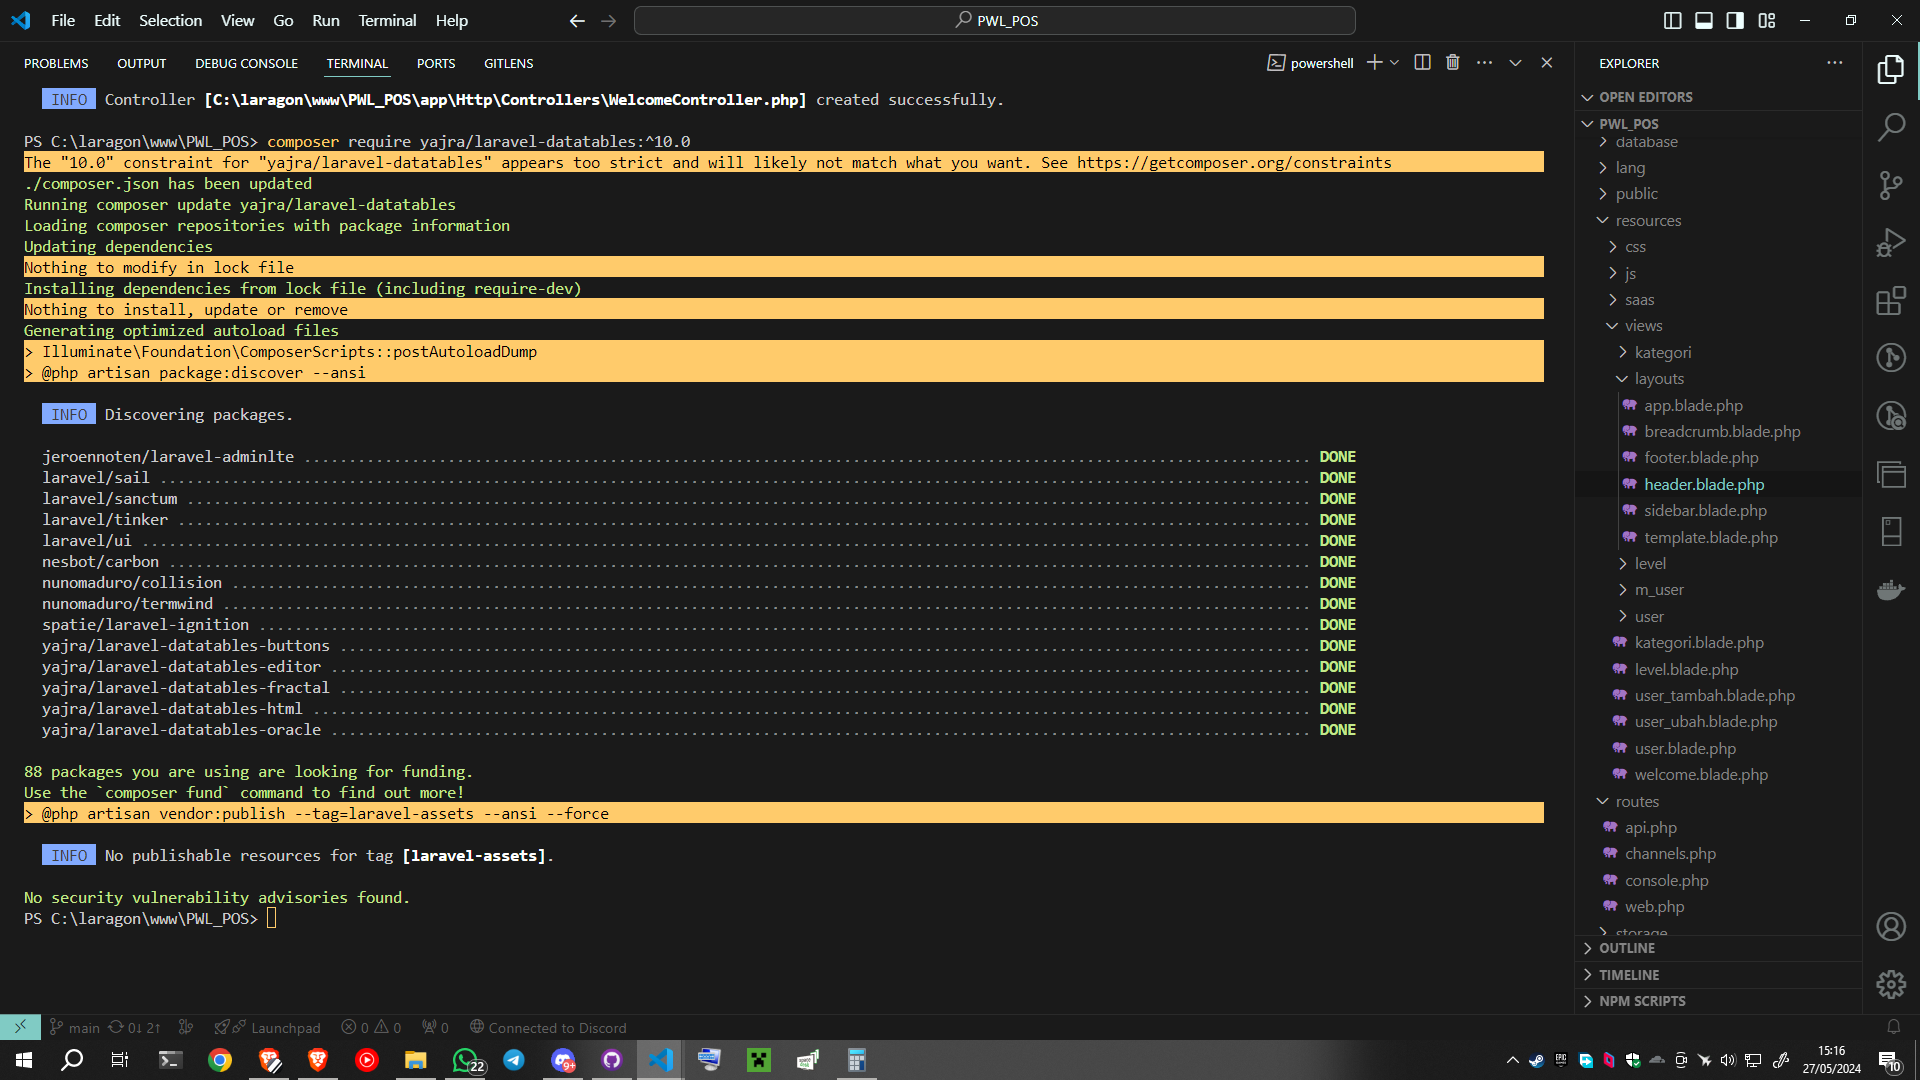
\includegraphics[width=.9\textwidth]{images/figures/Screenshot (461).png}
    \item[8.] - \\ 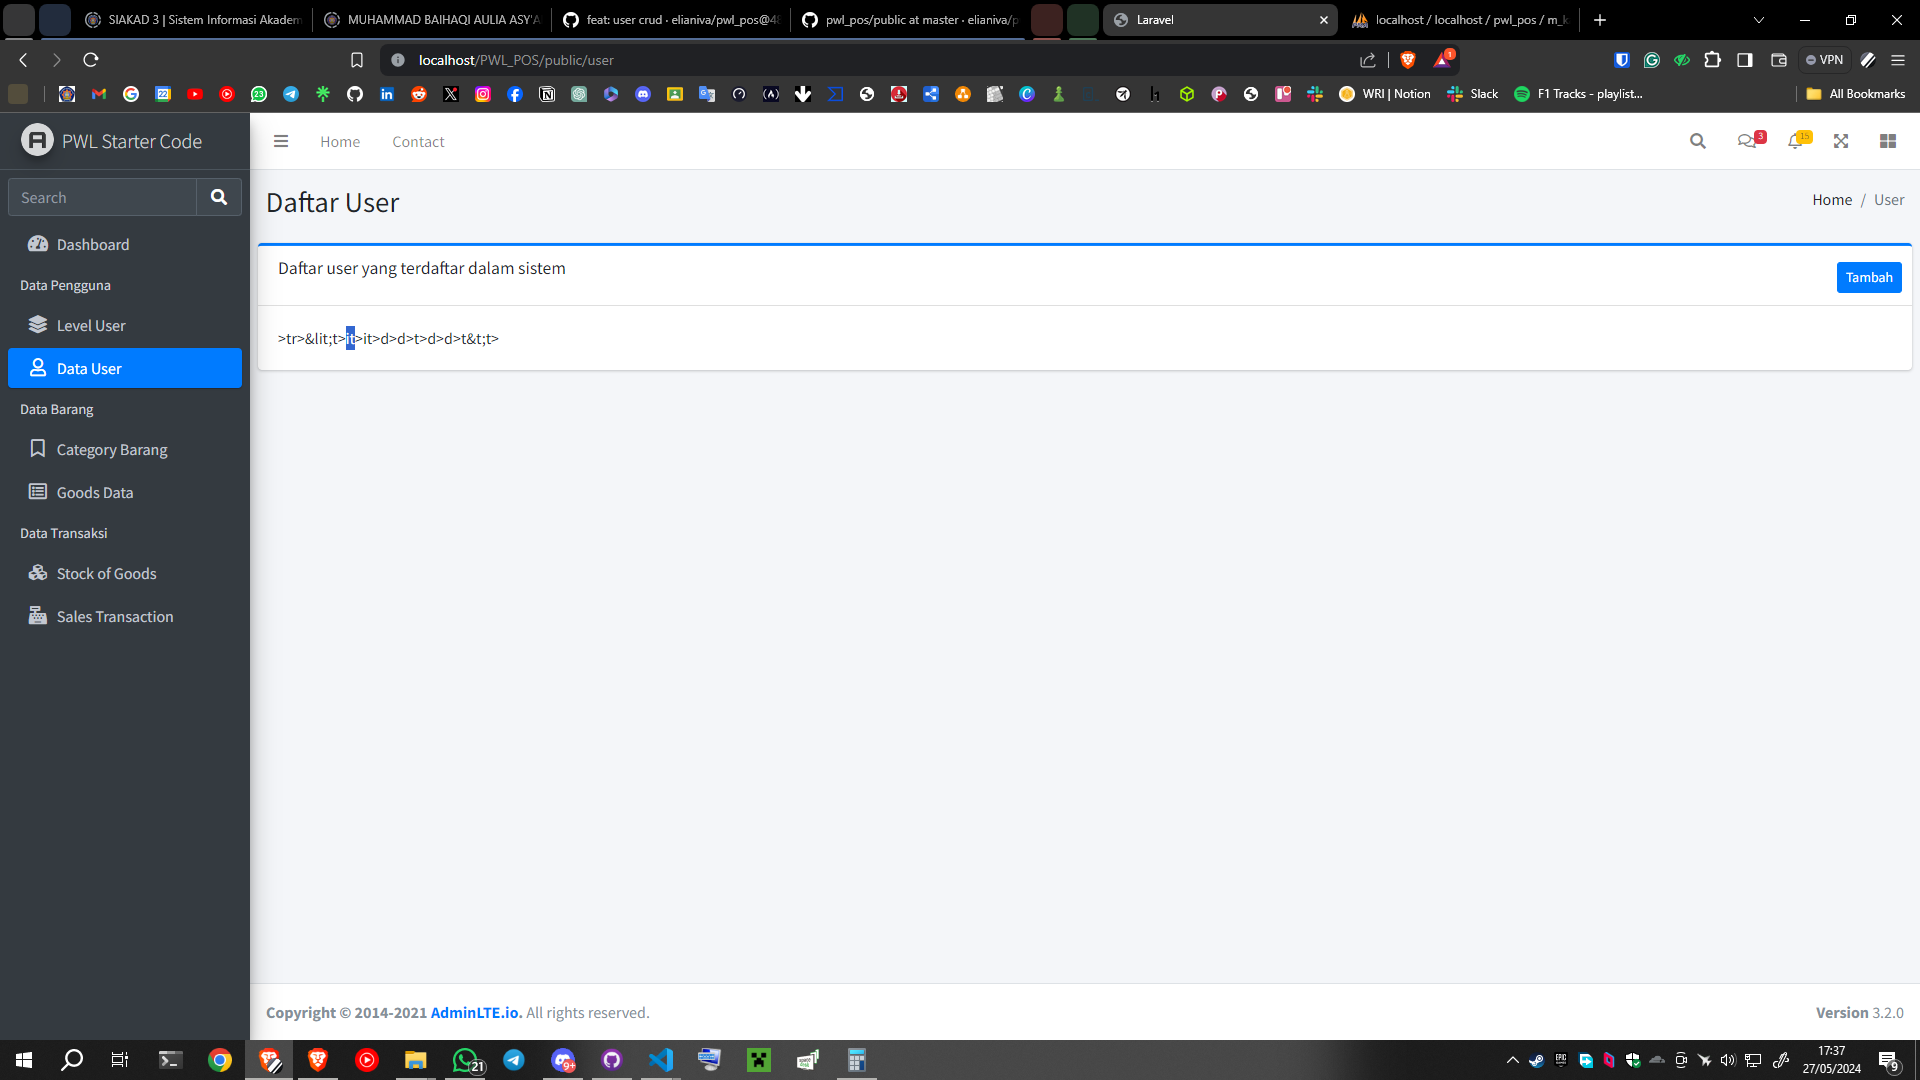
\includegraphics[width=.9\textwidth]{images/figures/Screenshot (462).png} \\ the template works but it has that one weird string
    \newpage
    \item[12.] - \\ 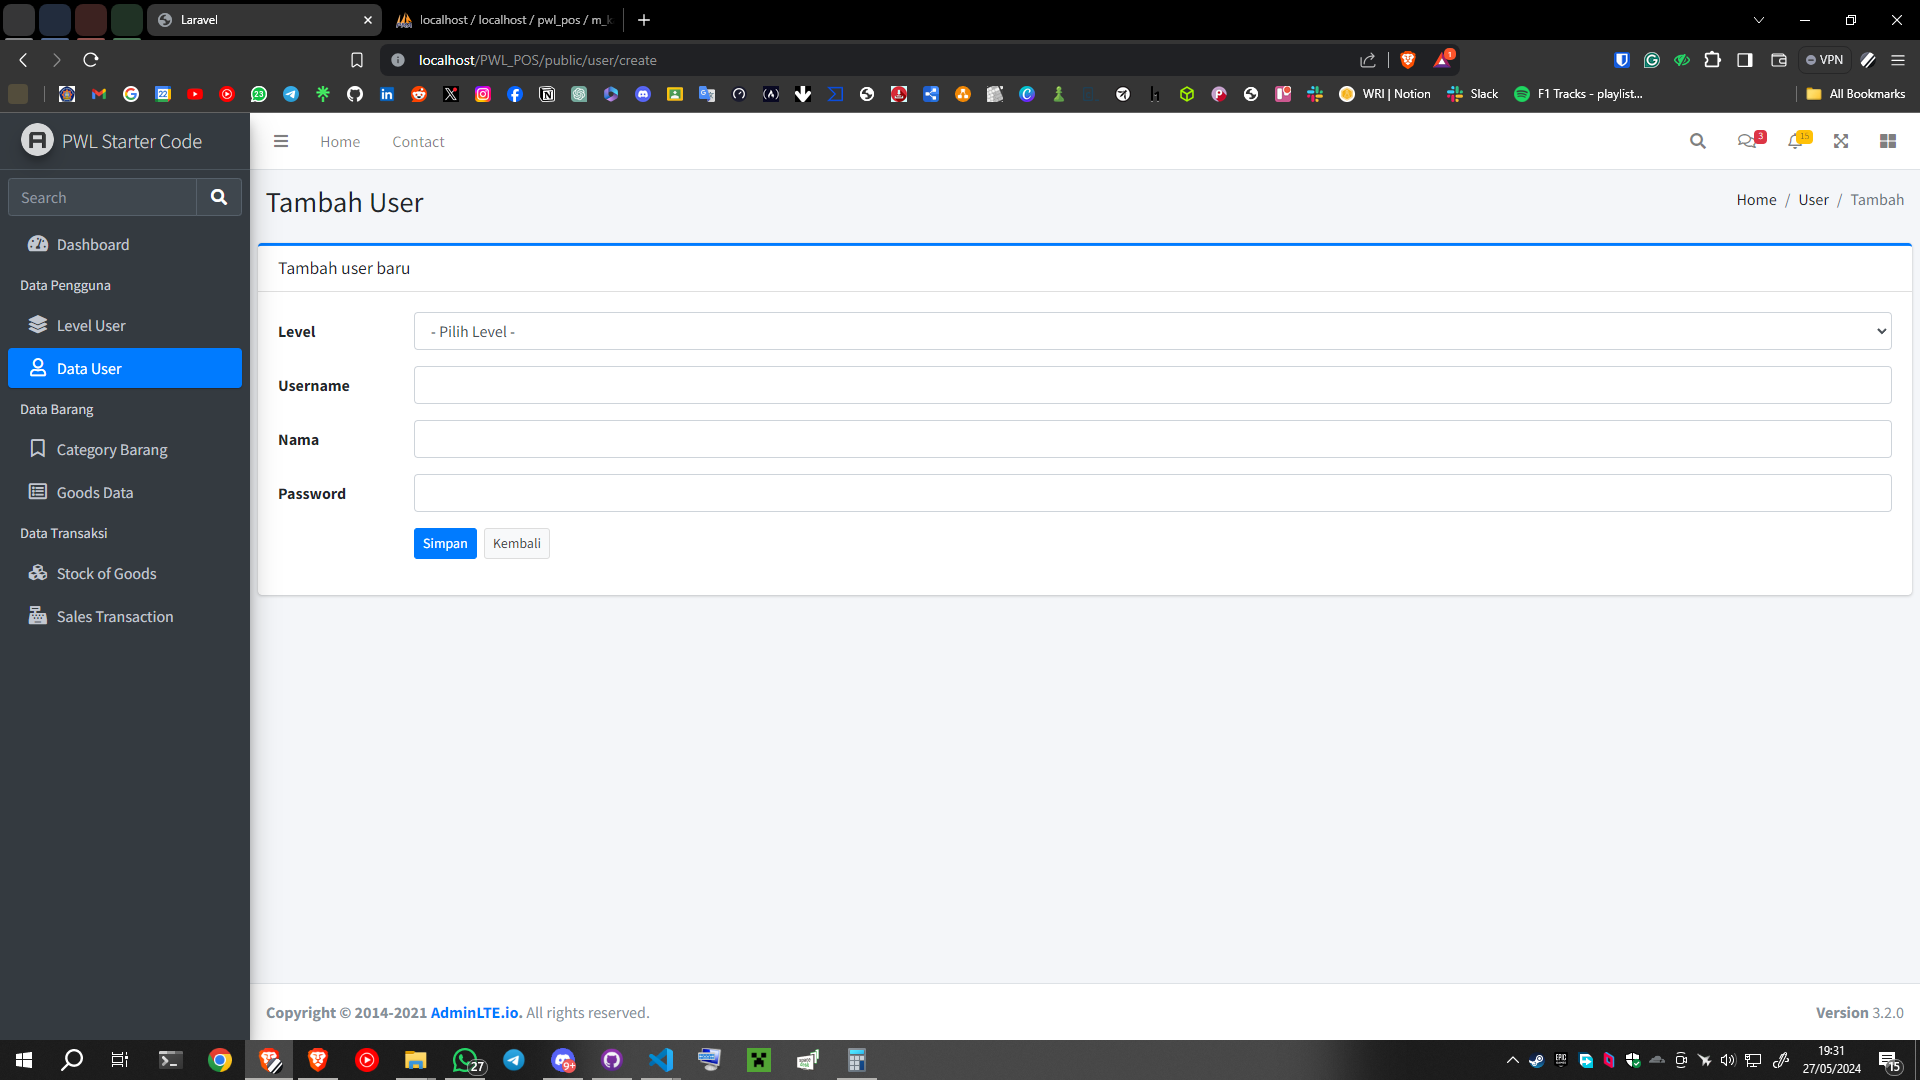
\includegraphics[width=.9\textwidth]{images/figures/Screenshot (463).png} \\ the create page looks more stylish and have a drop down menu for the level option
    \item[16.] - \\ \includegraphics[width=.9\textwidth]{images/figures/Screenshot (464).png} \\ it display an error because the user doesnt exist
    \newpage
    \item[20.] - \\ 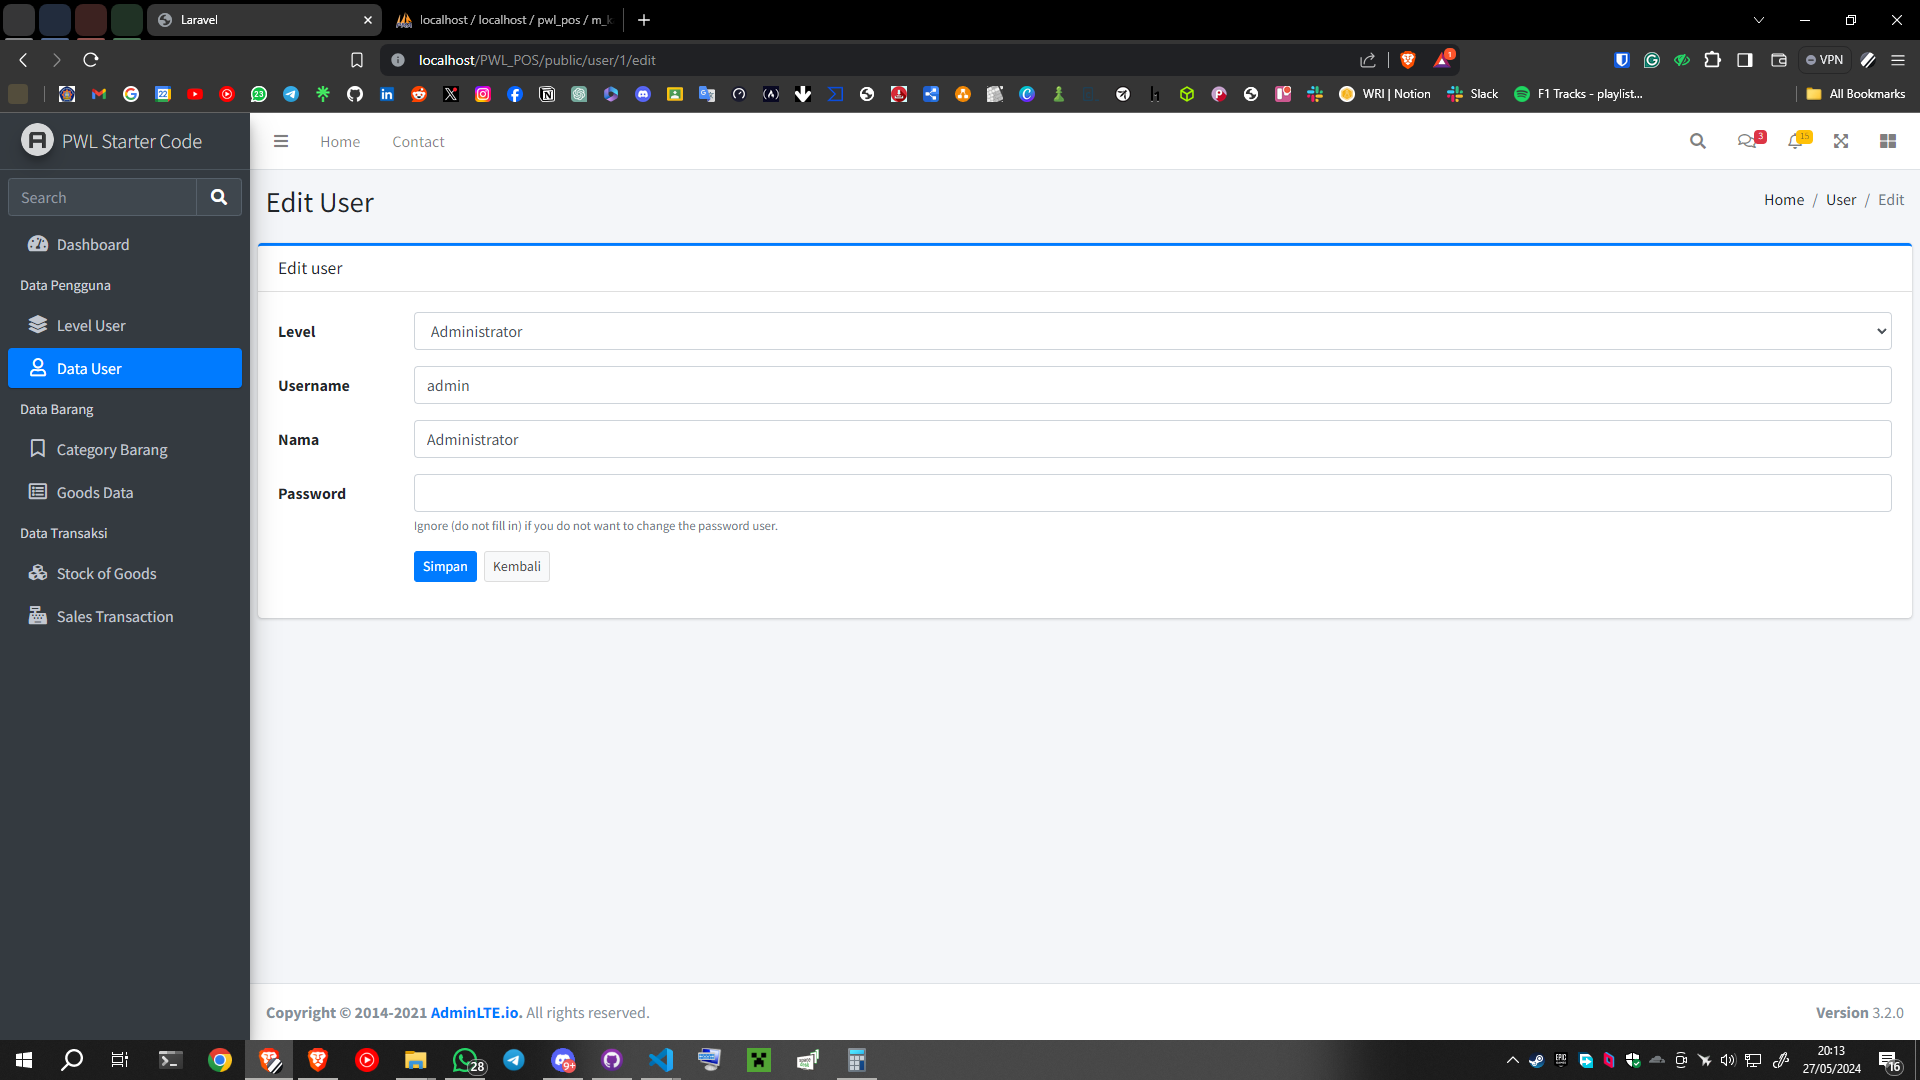
\includegraphics[width=.9\textwidth]{images/figures/Screenshot (465).png} \\ it is similar to the create page but now there is an already filled field
    \item[24.] - \\ 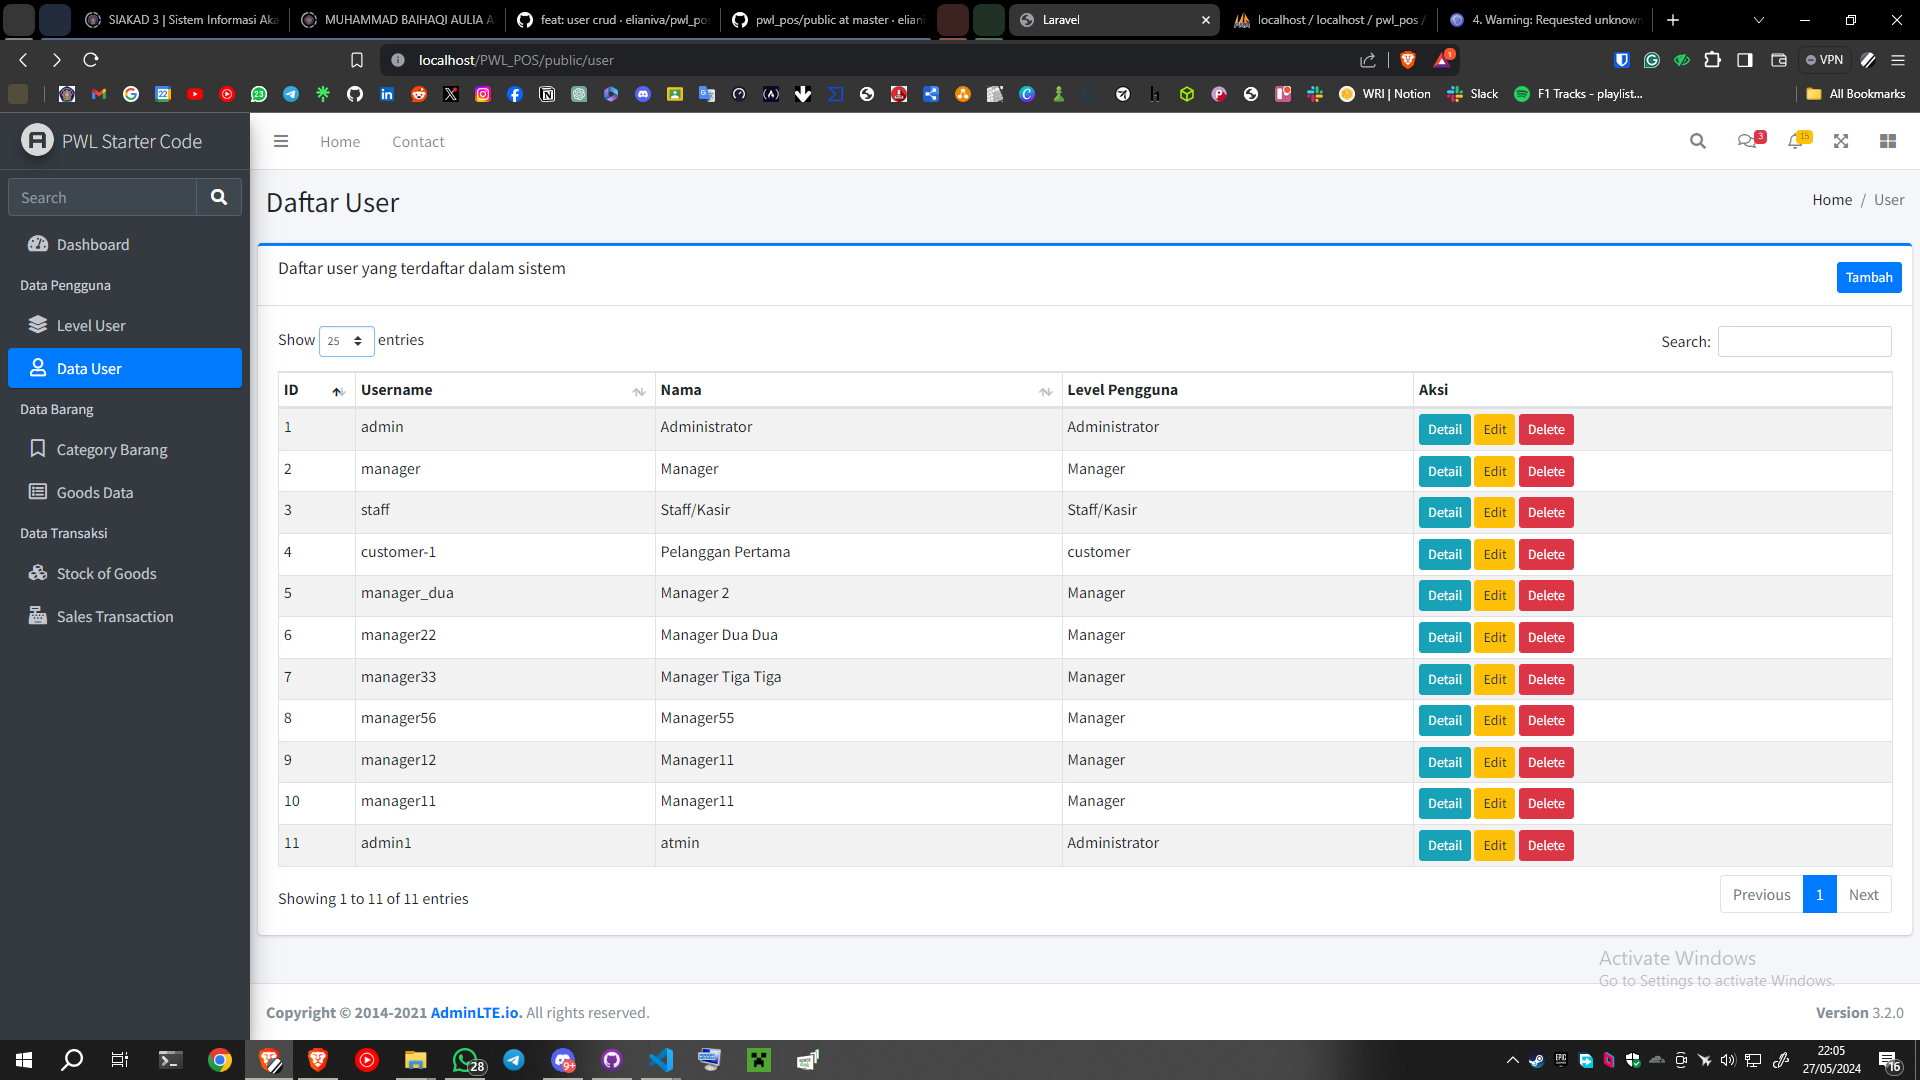
\includegraphics[width=.9\textwidth]{images/figures/Screenshot (469).png} \\ 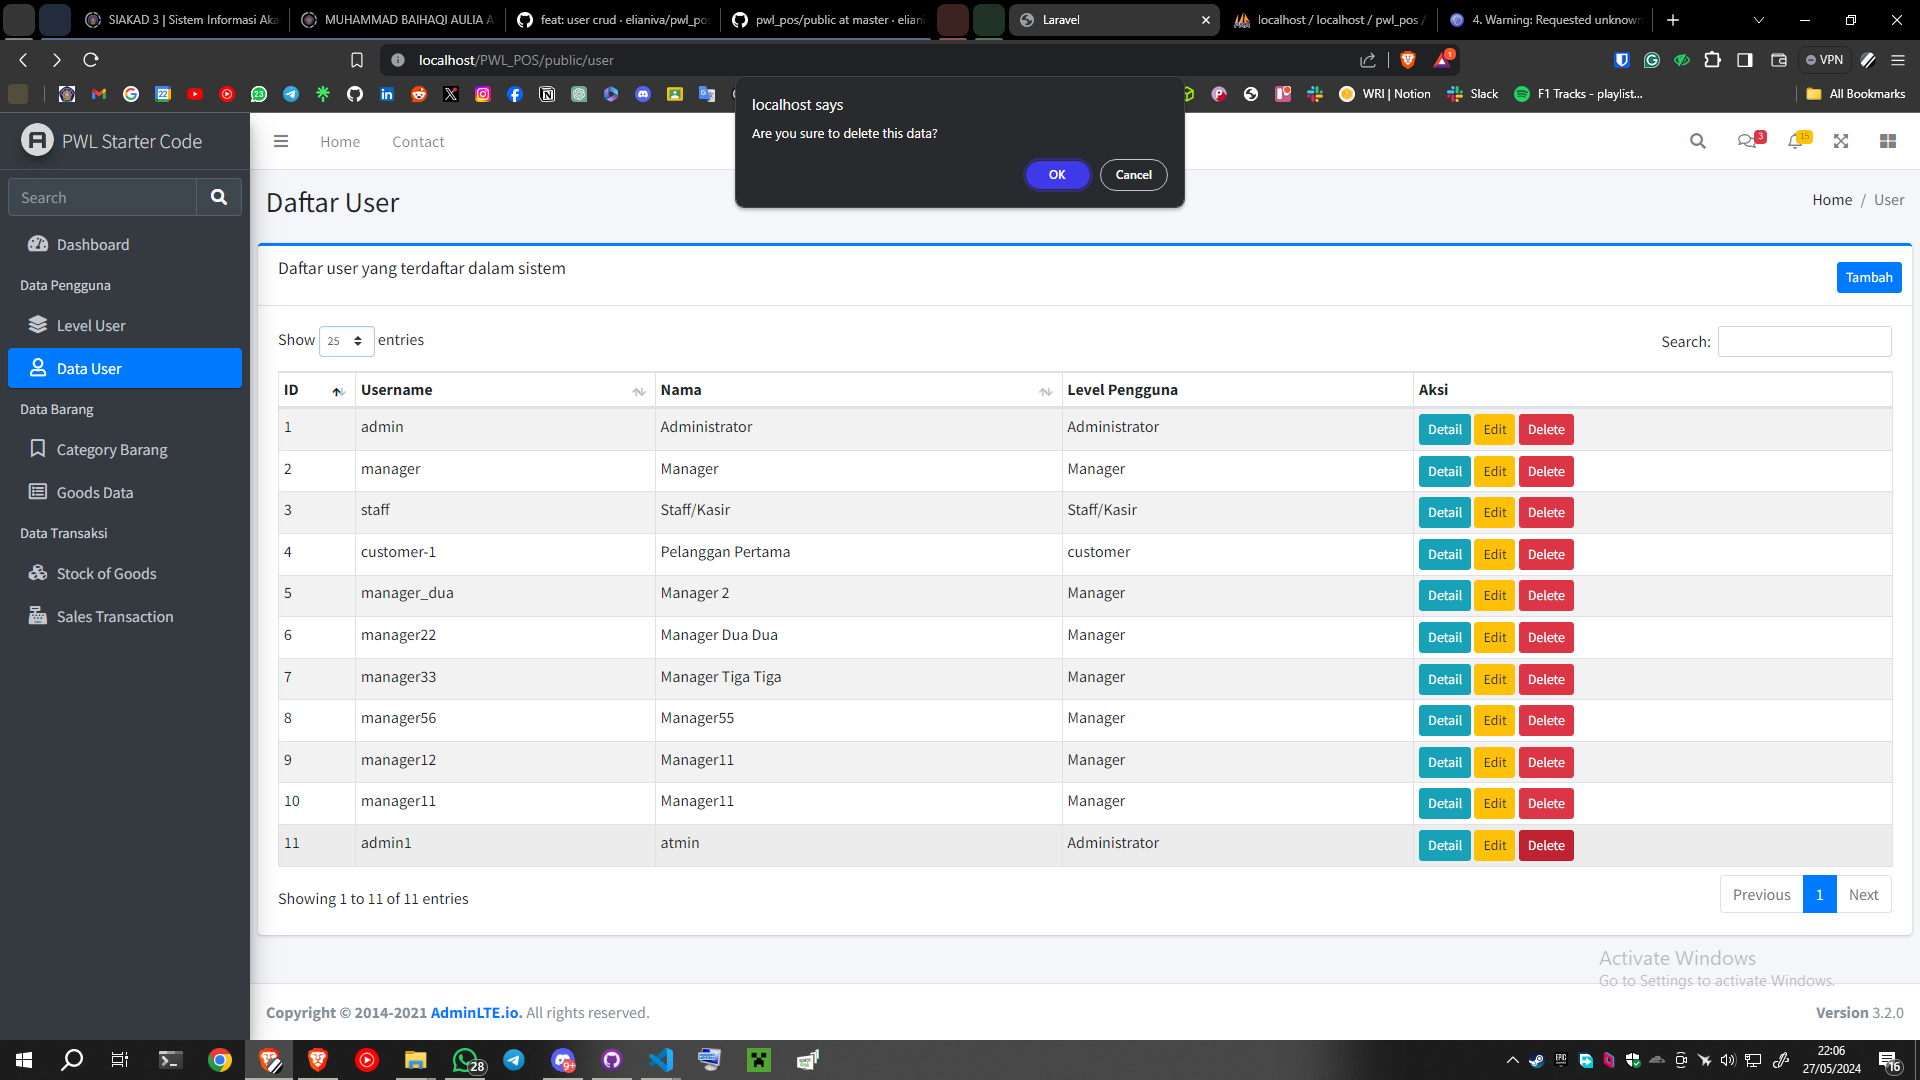
\includegraphics[width=.9\textwidth]{images/figures/Screenshot (470).png} \\ \includegraphics[width=.9\textwidth]{images/figures/Screenshot (471).png} \\ it confirm the decision before delete the user
\end{enumerate}
\newpage
\section*{Question}
\begin{enumerate}
    \item different type of user and layout
    \item yes, it simplify the building of a page
    \item include is when you want to add a chunk of ui element that is too big to be edited in one file. extend is to use the code as a template, effectively doing copy paste without the effort to do so. section is used to, in a way, store a ui element in a 'variable' that later can be use whenever a yield component is calling the variable. a push component is used for the css and js. a yield component can call on a section to use the ui component of the section. stack is used to bundle up css and js.
    \item is to indicate which sidebar nav to highlight
\end{enumerate}

\url{https://github.com/G4CENeiz/PWL_POS}

\end{document}